\documentclass{article}
\usepackage[a4paper]{geometry}
\usepackage{graphicx} % Required for inserting images
\usepackage[ruled,linesnumbered]{algorithm2e}
\usepackage{amssymb}
\usepackage{mathtools}
\usepackage{tikz}
\usepackage{quiver}
\usepackage{float}
\usetikzlibrary {cd,arrows.meta}

\usepackage{fontspec}
\setmainfont{EB Garamond}

\usepackage{amsthm}
\theoremstyle{plain}
\newtheorem{mytheorem}{Theorem}[section]
\newtheorem{mylemma}[mytheorem]{Lemma}
\newtheorem{myproposition}[mytheorem]{Proposition}
\newtheorem{mycorollary}[mytheorem]{Corollary}
\newtheorem{myconjecture}[mytheorem]{Conjecture}
%\theorembodyfont{\rmfamily}
\theoremstyle{definition}
\newtheorem{mydefinition}[mytheorem]{Definition}
\newtheorem{myassumption}[mytheorem]{Assumption}
% %\theoremstyle{remark}
\newtheorem{mynotation}[mytheorem]{Notation}
\newtheorem{myremark}[mytheorem]{Remark}
\newtheorem{myexample}[mytheorem]{Example}
\newenvironment{myproof}{\begin{proof}}{\end{proof}}
%\newtheorem*{myproof}{Proof}{\itshape}{\rmfamily}
\usepackage{hyperref}
\usepackage[colorinlistoftodos,prependcaption,textsize=tiny]{todonotes}
\newcommand{\dkcom}[2][1=]{\todo[linecolor=Plum,backgroundcolor=Plum!25,bordercolor=Plum,#1]{#2}}
\newcommand{\dknote}[2][1=]{\todo[linecolor=Plum,backgroundcolor=Plum!25,bordercolor=Plum,#1]{#2}}

\newcommand \id {\mathrm{id}}
\newcommand \tuple [1] {\left\langle #1 \right\rangle}

\title{Thoughts on hypergraphs for TERS}
\begin{document}
\maketitle



\begin{section}{Cool but maybe failed approach}
Idea: define TERS as a category, then consider string diagrams in that category.

Inspiration: \href{https://link.springer.com/content/pdf/10.1007/3-540-56393-8_2.pdf}{Context Rewriting, Stegan Kahrs} - they consider term rewrite system as a category enriched in a preorder, with objects - contexts, morphisms - terms, with ordering given by "t can be rewritten into g" iff $t \le g$ in the enrichment.


\begin{mydefinition}
    Define a category $T$ in the following way:
\begin{itemize}
    \item Objects are (lists of) contexts (lists are to allow finite products; everything is done pointwise)
    \item Morhisms are (lists of) terms.
\end{itemize}
Similar to \href{https://ncatlab.org/nlab/show/syntactic+category}{category of contexts}.
\end{mydefinition}

Attempt to reproduce the definitions from \cite{DBLP:conf/flops/MuroyaH24}

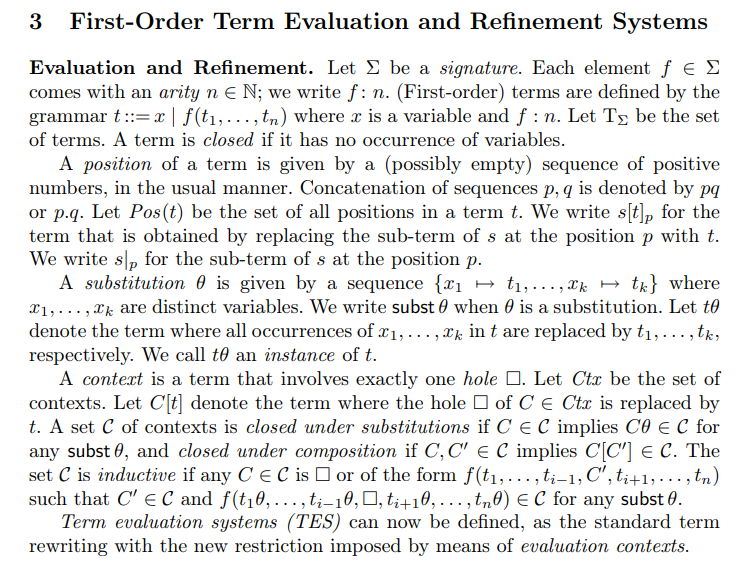
\includegraphics[scale=0.5]{images/ref.png}

\begin{itemize}
    \item substitution $t\theta$ is a composition of terms (values is a subset of all terms)
    \item {\color{red} context composition $C[C^{'}]$ ???}
    \item C[t] = $t(C)$ for morphism $t: C \rightarrow C^
    {'}$ for some $C^{'}$
    \item refinement and evaluation relations: whiskering? rule as a 2-cell (q: two different types of 2-cells for eval/refinement?)
    % https://tikzcd.yichuanshen.de/#N4Igdg9gJgpgziAXAbVABwnAlgFyxMJZABgBpiBdUkANwEMAbAVxiRAGEQBfU9TXfIRQBGclVqMWbbrxAZseAkQBMY6vWatEIbuJhQA5vCKgAZgCcIAWyRkQOCElETNbADpucACxg46Ms0sbRGcHJFUQACMYMCgkAFoAZjsGOmiGAAV+RSEQcywDLxwQdUktEAYSiqwwcrgIBiw46h86OMQwJgYGaj8sSu1IWqq4LyxTYpCeQOsnXsdECOjYpGTS121zKtT0rIVBNgYYCZGxk8RiLgouIA
\begin{tikzcd}
C \arrow[r, "\theta"] & {} \arrow[r, "l"', bend right, shift right] \arrow[r, "r", bend left] & {}
\end{tikzcd}

Evaluation rules are certain rewrites $l \rightarrow r$. The evaluation relation $\rightarrow_{\epsilon}$ for TES requires for every such rule and for every evaluation context C, to have $C[l\theta] \rightarrow_{\epsilon} C[r\theta]$. 
\end{itemize}

Conclusion: need to define $C[C^{'}]$, then define TES, then introduce a second set of rules (refinement) to get TERS.

Questions: we have two kinds of rewrites, both between the same terms. Is it two different enrichements? 
Enrichment in a double category?

\end{section}
\begin{section}{A better approach}
Alternatively, just follow the same approach as with terms.

A hypergraph with a hole <=> a hypergraph with a chosen subgraph up to equivalence.

\begin{mydefinition}
    A context in $Hyp_{\Sigma}$ is an equivalence class of monomorphisms $C: H \rightarrow G$, where $C \equiv C'$ when $H, H'$ have the same interface and the images in $G, G'$ of the interface are also the same. $G \backslash H = G' \backslash H'$.
\end{mydefinition}

A composition of contexts $C_1[C_2]$ with $C_1: H_1 \rightarrow G_1$ and $C_2: H_2 \rightarrow G_2$ is possible when $G_2$ and $H_1$ have the same interface. The interface of the resulting hole is (the one of) $H_2$.

\[C_1[C_2]: H_2 \rightarrow G_2 \equiv H_1 \rightarrow G_1\].

\begin{mydefinition}
    A substitution $\theta: [x] \rightarrow [t]$ is a morphism sending variables to terms. 
\end{mydefinition}

\begin{mydefinition}
    A set of contexts $\mathcal{C}$ is closed under substitution if $C: H \rightarrow G \ \in \mathcal{C}$ implies $C\theta: \theta(H) \rightarrow \theta(G) \in \mathcal{C}$ for every substitution $\theta$.
\end{mydefinition}

Now, the definition of first-order TES (HES? Hypergraph Evaluation System) stays the same.


\begin{figure}[H]
\hspace{-1.0cm}
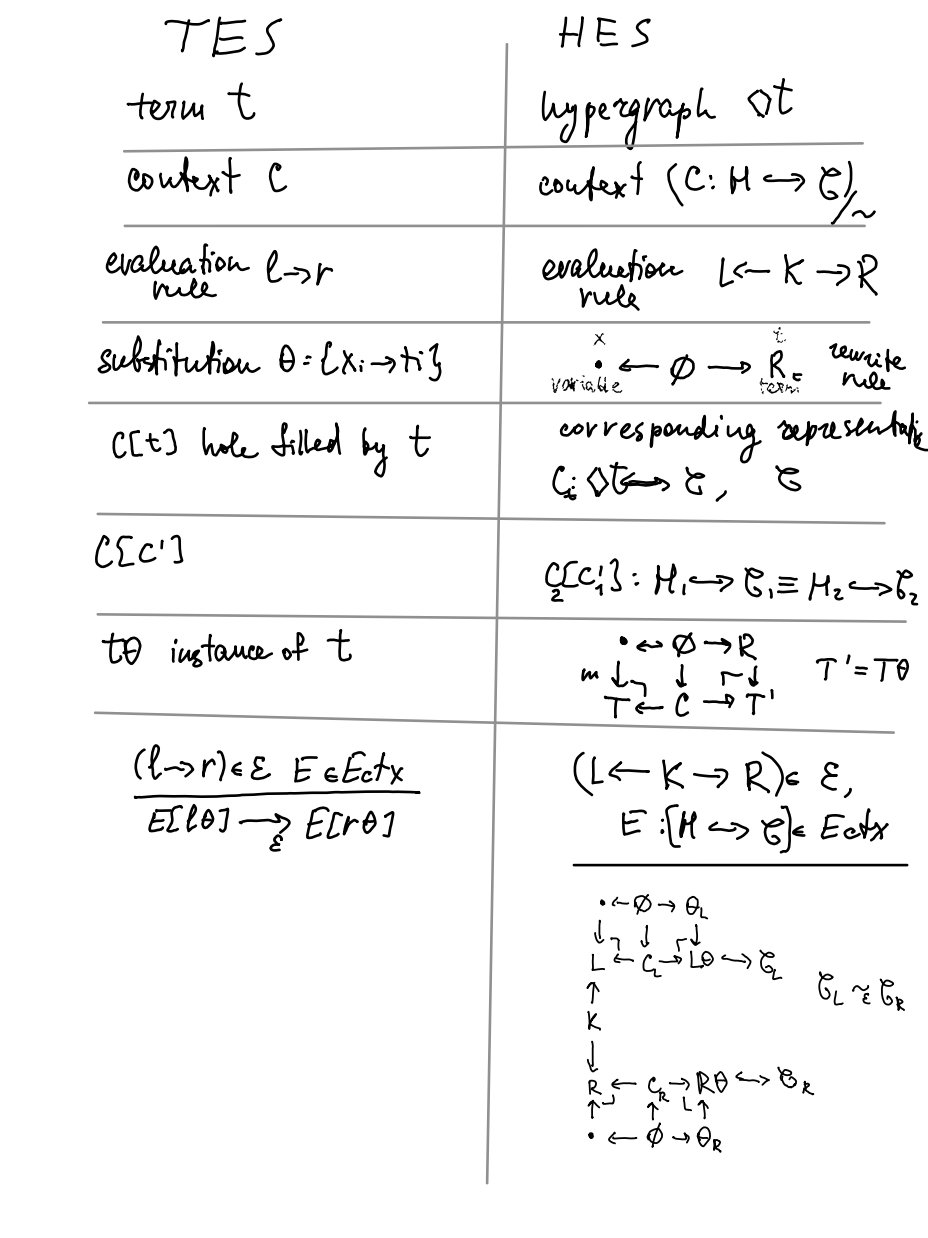
\includegraphics[scale=0.8]{images/teshes.png}
\caption{Comparison of definitions of TES and HES}
\end{figure}

Next are definitions for peaks and appropriate joinability for HERS.

\begin{figure}[H]
%\hspace{-1.0cm}
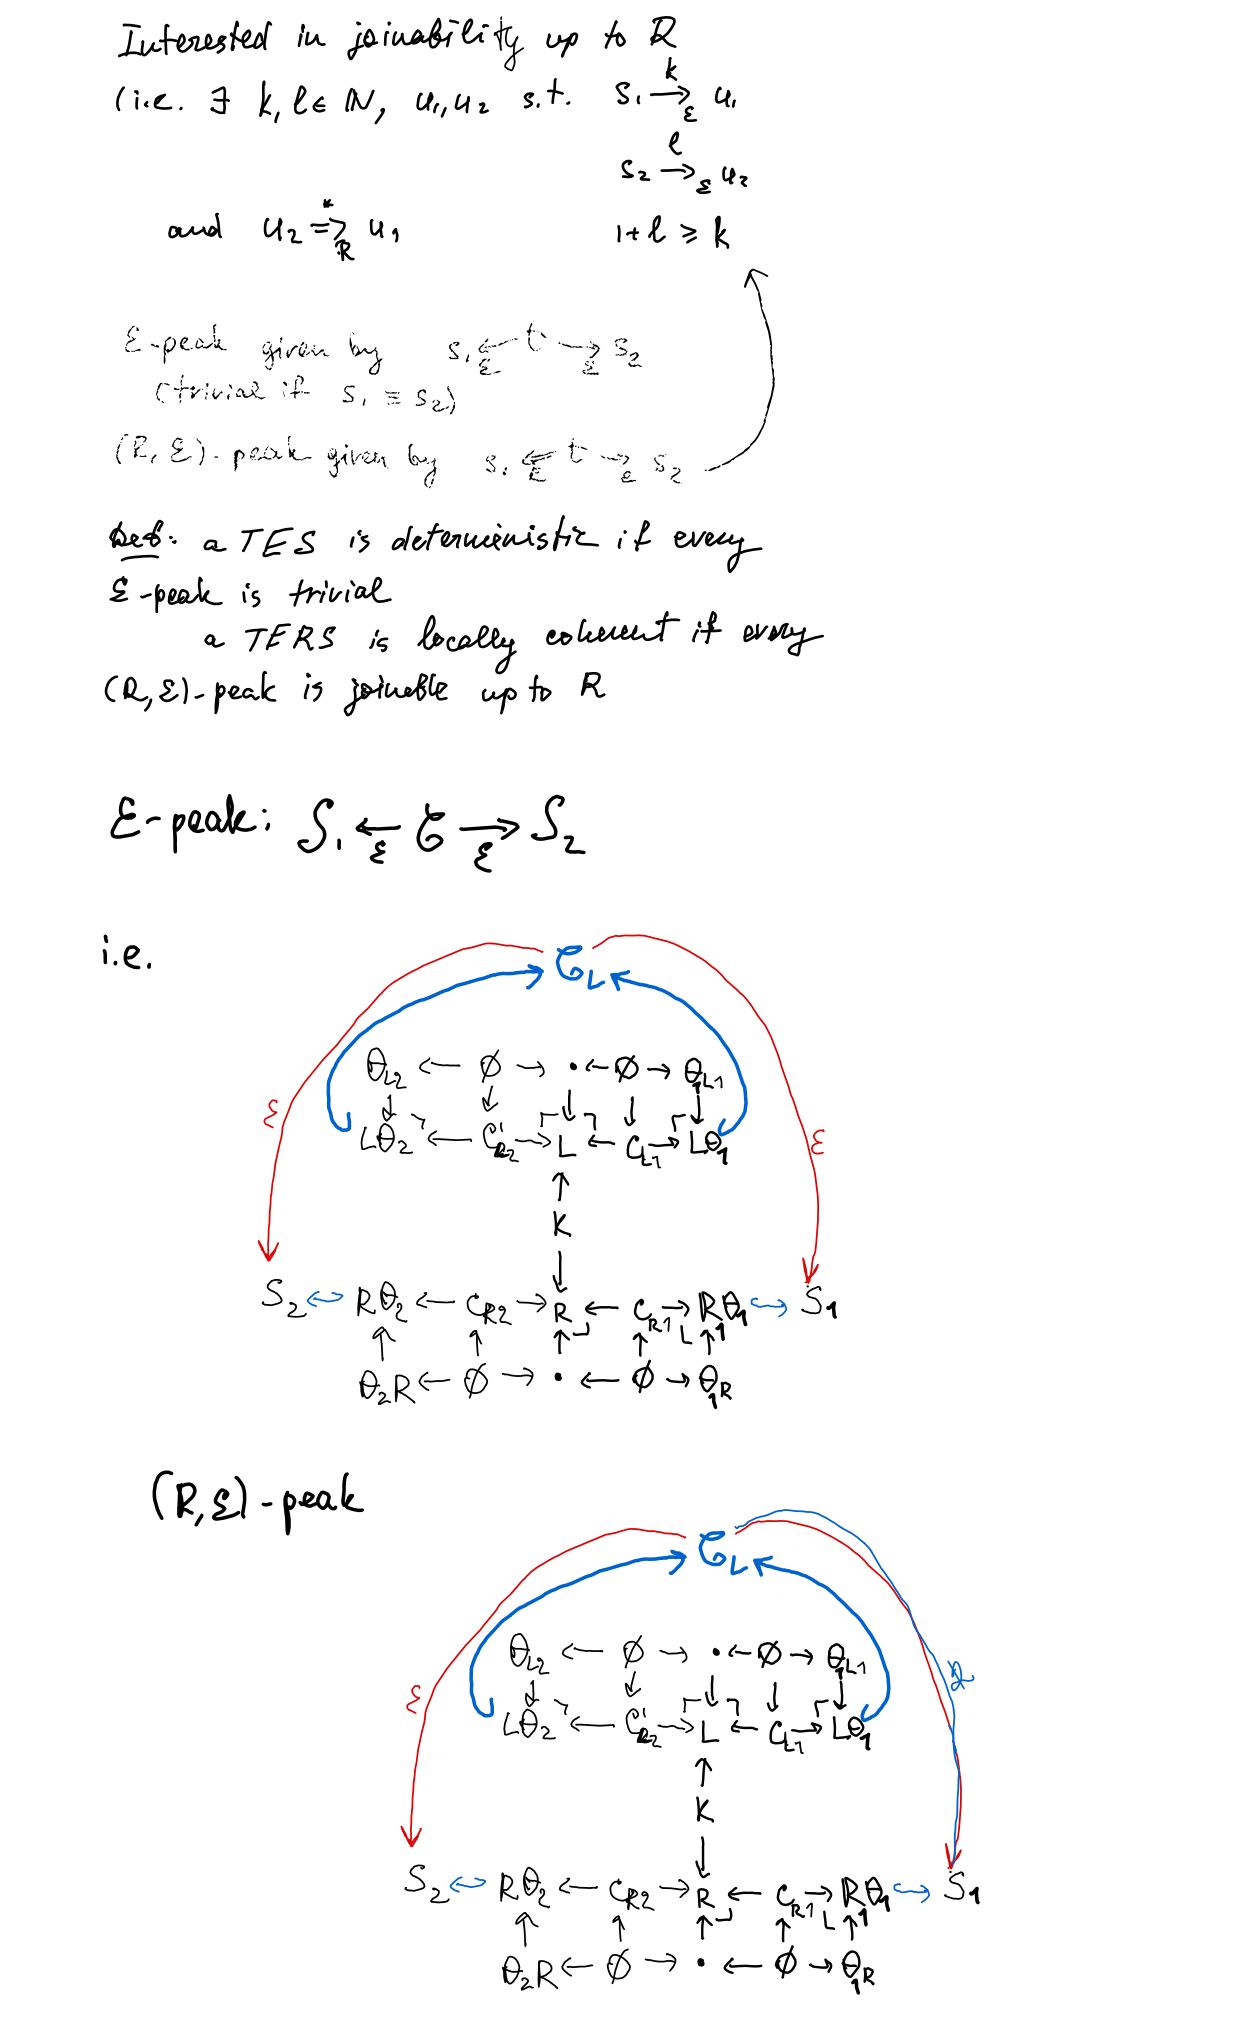
\includegraphics[scale=0.8]{images/peaks.png}
\caption{Peaks for HERS}
\end{figure}

\begin{figure}[H]
\hspace{-1.0cm}
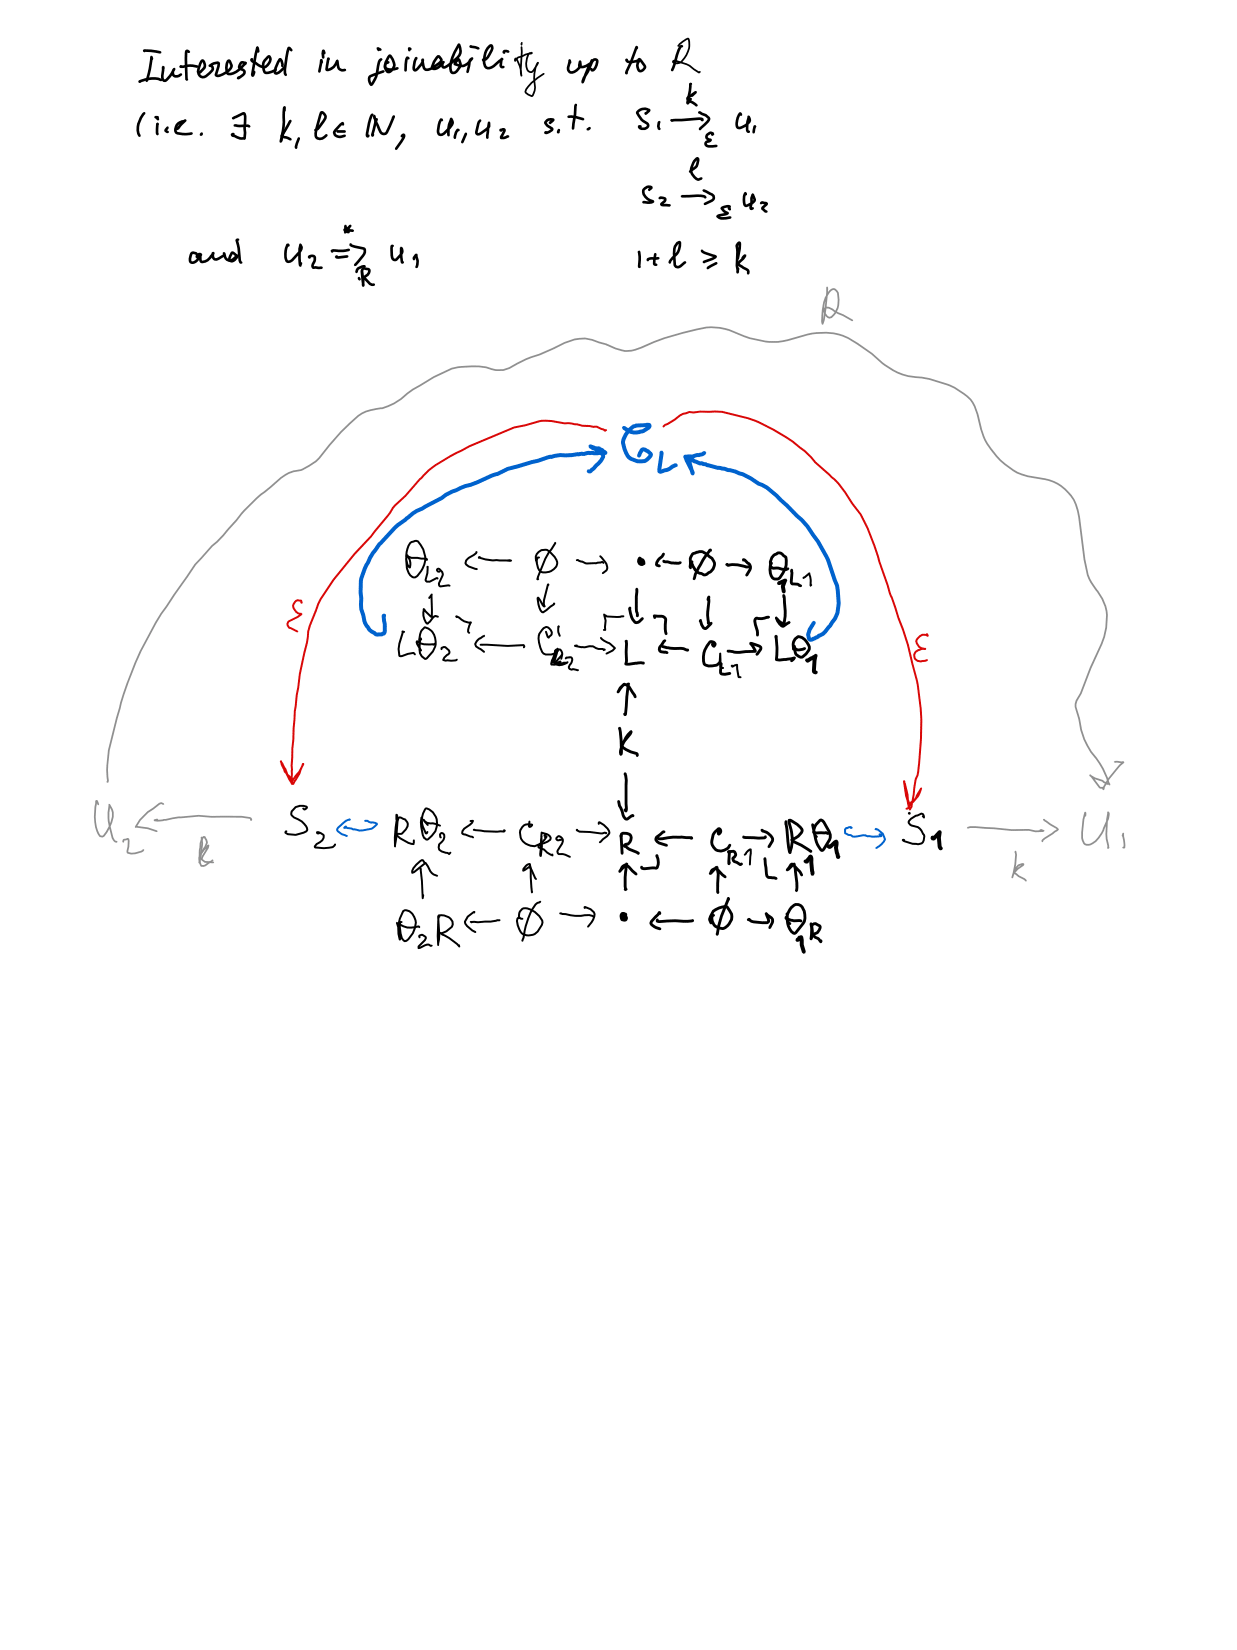
\includegraphics[scale=0.8]{images/joinuptor.png}
\caption{Joinability up to $\mathcal{R}$ for HERS}
\end{figure}

\begin{subsection}{Second Order TERS}
Idea: meta-level = hierarchical hypergraphs

Intuition for metavariable - placeholder of a certain shape for a hypergraph, arity is the number of arguments it can take. 1st level term embedded into a 2nd level graph. That's why layers make sense, next layer variable = previous layer term.

Then metaterm is a hypergraph that has metavariables, i.e. hypergraph with layers. 

{\color{red} variable binding for hypergraphs? what does "x.t" mean here?}

$M[t_1, \dots t_m]$ - arguments are substitutions for metavariables; i.e. for the layer corresponding to M, fill it with hypergraphs $t_1, \dots t_m$ at the corresponding places.


So far it is still term graphs and not really hypergraphs, how to let go of that dependency...

Next is example from the paper but with pictures! (I couldn't find the usual way to represent $\lambda$ calculus in hypergraphs)
\begin{subsubsection}{Example CBV$\lambda$}
\begin{figure}[H]
\hspace{-1.0cm}
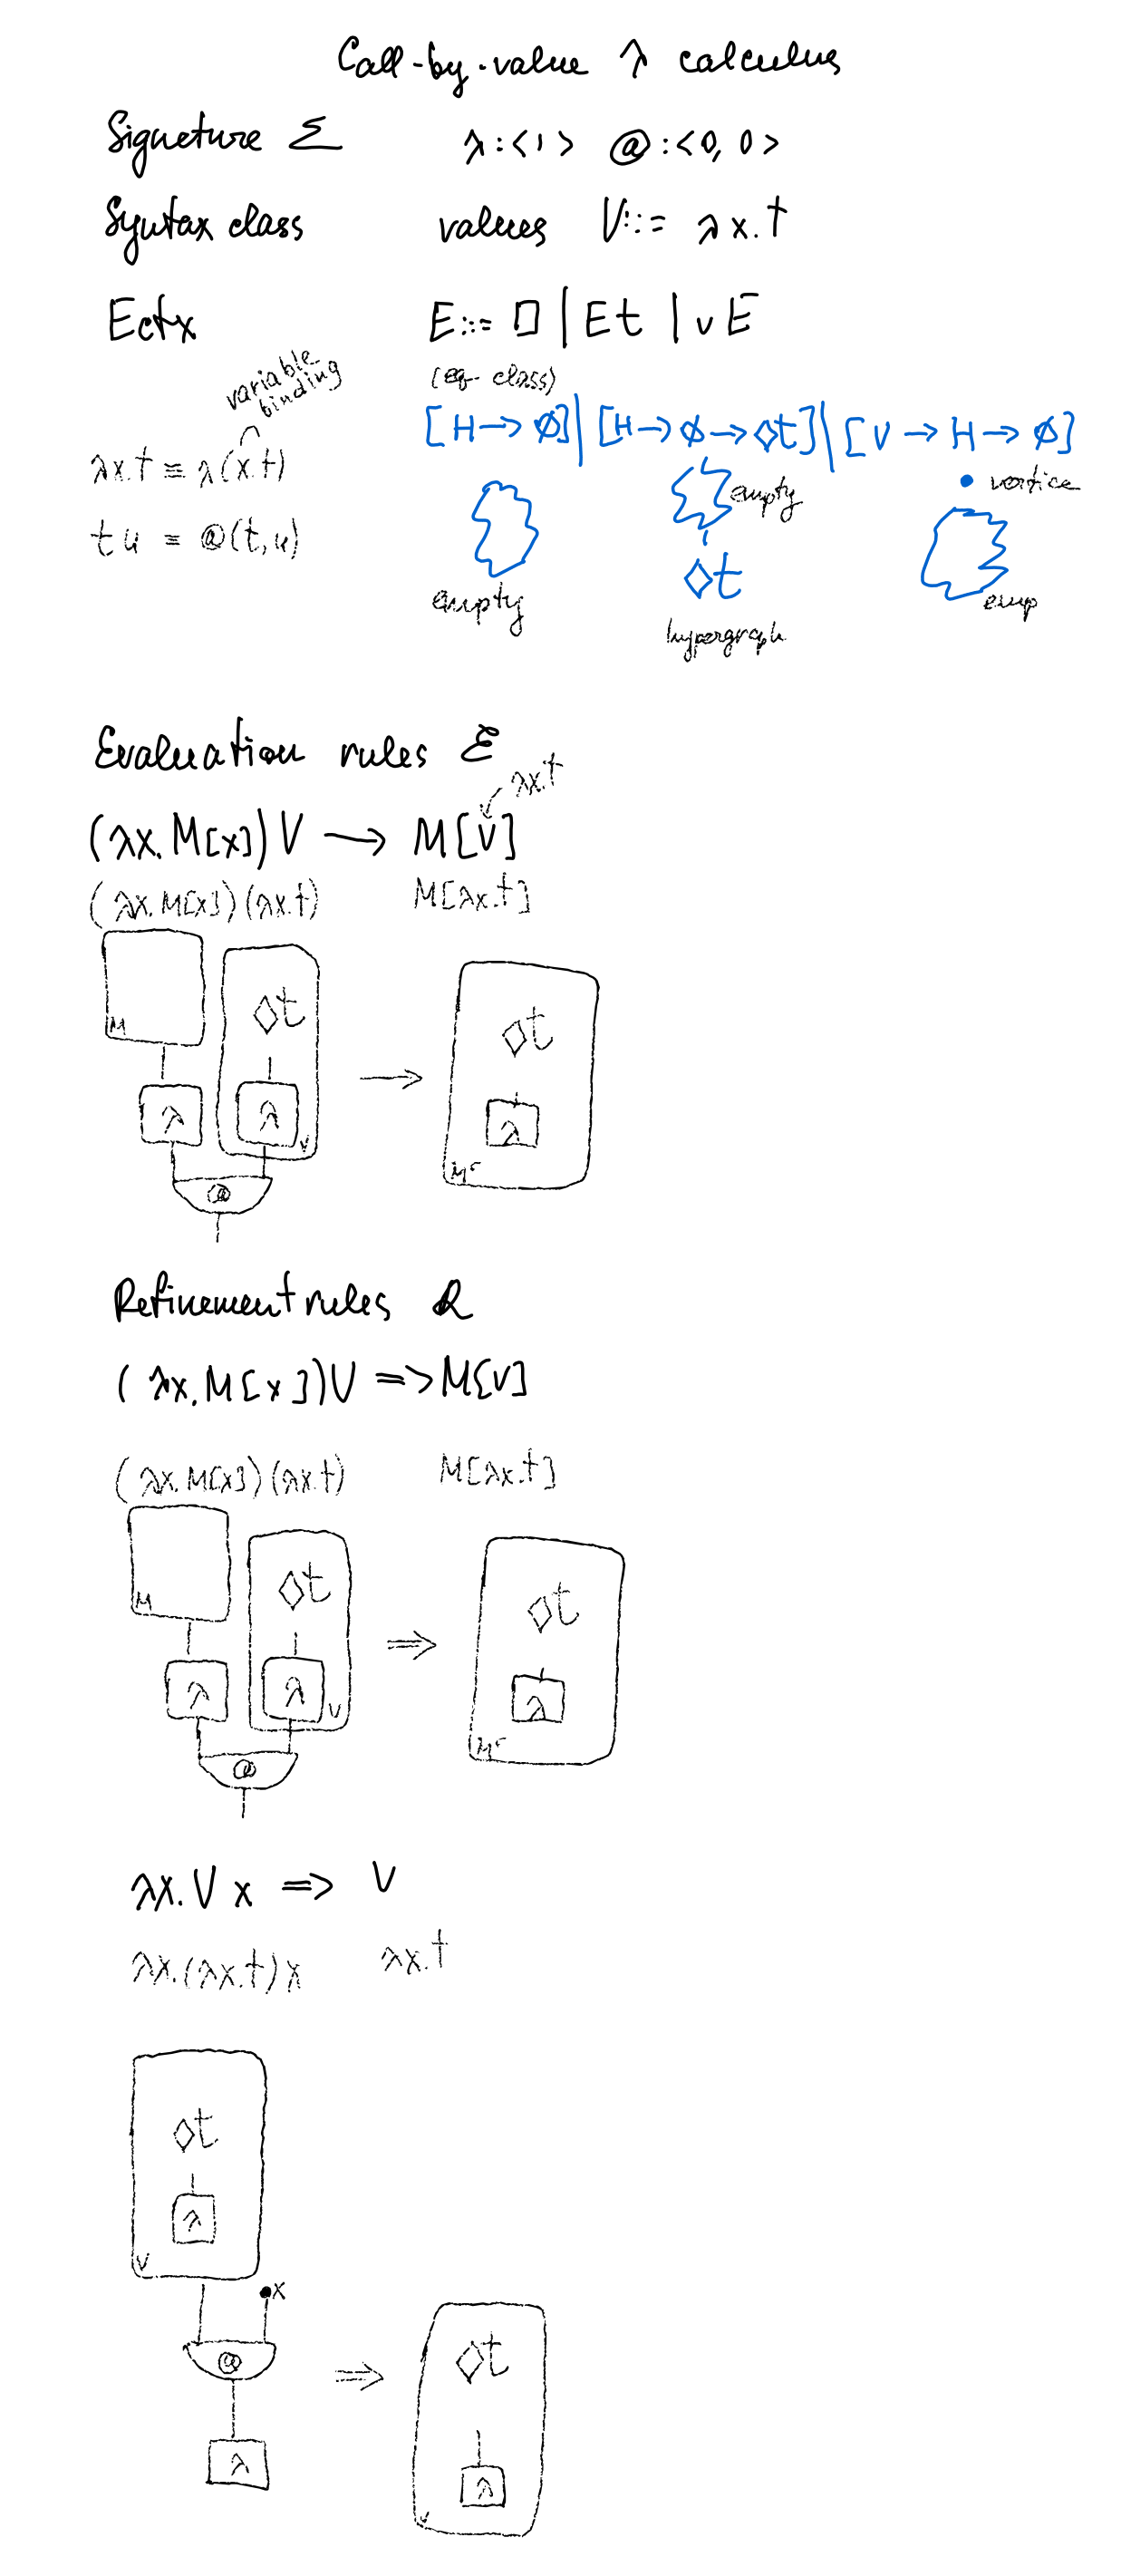
\includegraphics[scale=0.7]{images/cbvl.png}
\caption{CBV$\lambda$ example}
\end{figure}

\end{subsubsection}

\end{subsection}

\end{section}

\begin{section}{Other possibly related papers}
EGG library \href{https://pavpanchekha.com/blog/egg-bindings.html}{The egg project uses e-graphs to provide a new way to build program optimizers and synthesizers}.

I have seen several papers with implementation in HyperLMNtal, might be something of interest as well. 
\href{https://ieeexplore.ieee.org/stamp/stamp.jsp?tp=&arnumber=7541894}{$\lambda$ calculus}
\href{https://www.jstage.jst.go.jp/article/transinf/E101.D/4/E101.D_2017EDP7257/_pdf/-char/en}{Name binding} 

\href{https://link.springer.com/article/10.1007/s13218-011-0162-3}{HyperLMNtal - Hierarchical Graph Rewriting Model}
    
\end{section}
\bibliographystyle{apalike}
\bibliography{ref}
\end{document}